%%%%%%%%%%%%%%%%%%%%%%%%%%%%%%%%%%%%%%%%%%%%%%%%%%%%%%%%%%%%%%%%%%%%%%%%%%%%%%%%
%2345678901234567890123456789012345678901234567890123456789012345678901234567890
%        1         2         3         4         5         6         7         8
% THESIS CHAPTER


\chapter{Vision: Methods \& Results}
\label{chap:vision}
\ifpdf
    \graphicspath{{Vision/Figures/PNG/}{Vision/Figures/PDF/}{Vision/Figures/}}
\else
    \graphicspath{{Vision/Figures/EPS/}{Vision/Figures/}}
\fi

\begin{figure}[H]
	\centering
	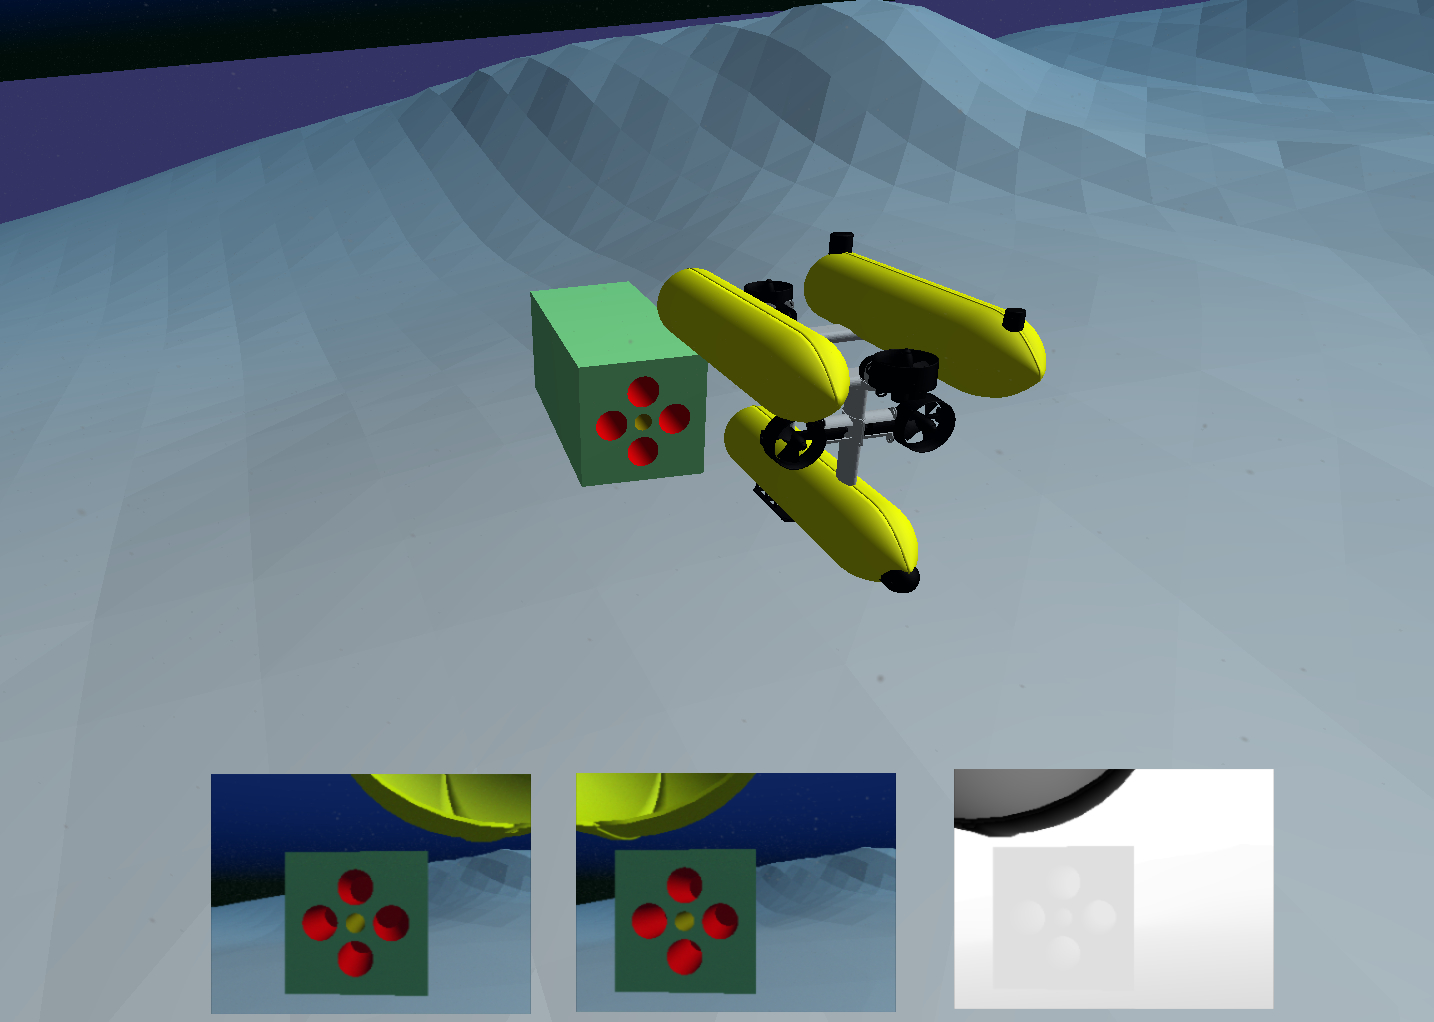
\includegraphics[width=13.5cm]{Vision_uwsim.jpeg}
	\caption[The Vision robot watching the hole]{The \textit{vision} Robot watching the hole. The hole (in yellow) is in the centre of the cuboid. The red holes around are there to help vision algorithms. Below, the right RGB, the left RGB and the left depth cameras are shown. In the methods, only one of the left cameras is used.}
	\label{fig:vision-uwsim}
\end{figure}

This Chapter covers exclusively the Vision part. So, here they are presented methods and tools to estimate the hole's position with computer vision algorithms. To not go outside the scope of this thesis, the methods are only introduced, briefly explained, and compared; no theoretical background is given. So, no mathematical formulas are illustrated for the used vision functions. \\

Before the two carrying robots can approach the hole, obviously the hole's position must be know, at least roughly.
In the considered scenario, a third robot is present, as depicted in figure \ref{fig:vision-uwsim}. Its work is devoted exclusively \textit{to detect} and \textit{to track} the hole. In the simulation, another \href{https://cirs.udg.edu/auvs-technology/auvs/girona-500-auv/}{Girona 500 AUV} is used for this job, without the arm. It is evident that, in a real scenario, a smaller and more efficient robot should be used for the vision, seeing that no manipulation capability are needed. In fact, in the original TWINBOT [\cite{TWINBOT2019}] simulation, a smaller \href{https://bluerobotics.com/product-category/rov/bluerov2/}{BlueROV} is present.
Anyway, for this thesis, another Girona 500 is used to not deal with an additional robot model.\\

\begin{figure}[H]
	\centering
	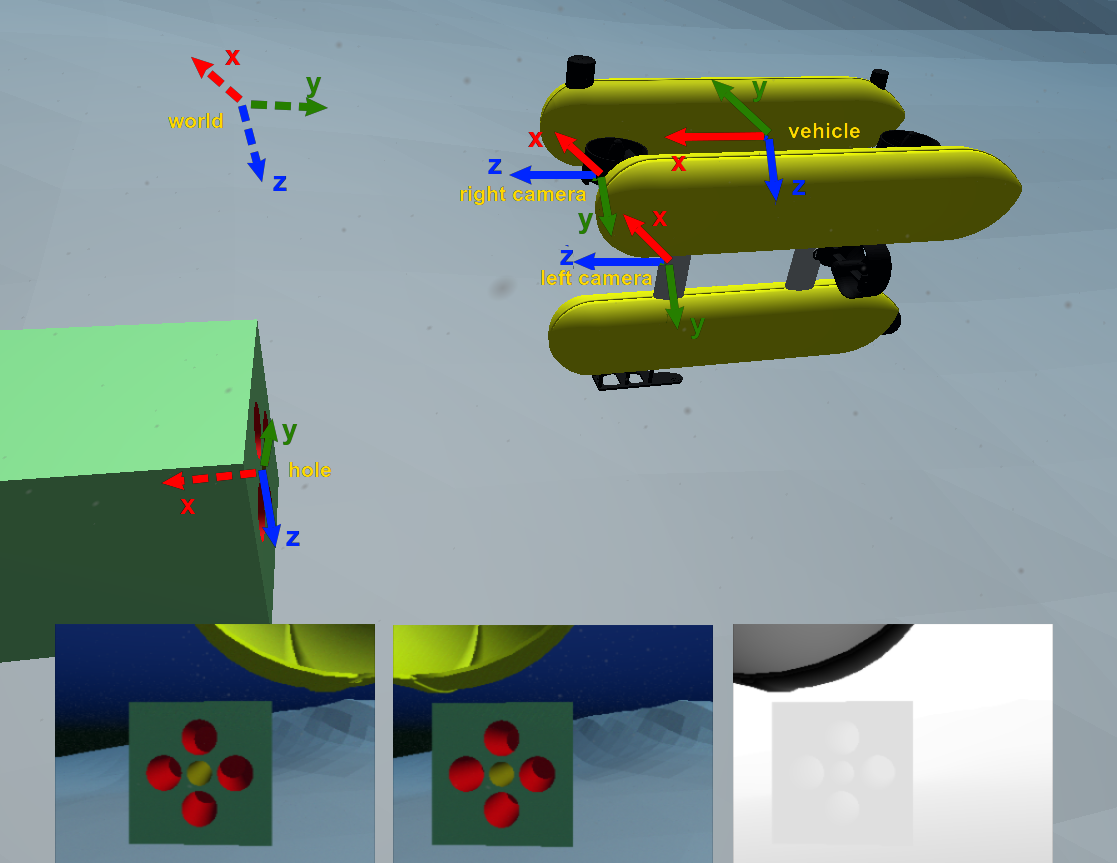
\includegraphics[width=12.5cm]{frameVision.png}
	\caption[Main frames of the Vision scenario]{Screenshot where the main frames for the Vision are depicted. The cameras 3D models are not present. The left and the right cameras have same orientation, and the origin of the right one is shifted of 0.2 meters along left camera's $x$-axis. Vehicle and cameras axis are parallel. Hole's $x$-axis goes inside the cavity. World's frame is depicted only to understand its orientation, its origin is not in that point.}
	\label{fig:visionFrames}
\end{figure}

The Vision robot is equipped with two cameras which point in front of it, as shown in figure \ref{fig:visionFrames}. They are used for three different methods as:
\begin{itemize}
	\item Two distinct cameras, independent of each other (mono camera case).
	\item As stereo cameras, thus exploiting stereo vision algorithms.
	\item As RGB-D camera, i.e., a stereo vision couple where the left one is a RGB camera and the right one is a Depth camera.  
\end{itemize} 

\noindent The job is divided in two phases: \textit{Detection}  of the hole (section \ref{sec:visDetect}) and \textit{Tracking} of the hole's pose \mbox{(section \ref{sec:visTracking}).} 

\section{Assumptions}
\label{sec:visioAssumption} %cited by method chapter in assumption section
For the sake of simplicity, some assumptions are made:
\begin{itemize}
	\item Known \textit{intrinsic} camera parameters. These parameters are used by algorithms to take into account how the single camera sees the scene. No image distortion is present.
	\item Known \textit{extrinsic} camera parameters, i.e. the position and the orientation of cameras (respect to the vehicle), and thus it is also known the relative pose between the two cameras (needed for stereo vision algorithm).
	\item No external disturbances for Vision, such as underwater light reflections or bad visibility.
	\item Hole's model known. This means that dimensions of the cuboid which contains the hole are known. Further explanation about this are given successively in section \ref{sec:visTracking}.
	\item A "friendly" cuboid structure of the hole. The front face is coloured and additional holes are present, as can be seen in fig. \ref{fig:vision-uwsim}. This helps both the \textit{detection} phase and the \textit{tracking} phase.
\end{itemize}
About the robot, other assumption are:
\begin{itemize}
	\item The pose of the vehicle respect to the inertial frame (the \textit{world}) is known. This is important to share the hole's pose with the carrying agents. Further details about this are given in section \ref{sec:expAssumption}.
	
	\item The initial position of the robot is such that it is facing the front face of the hole. It must be noticed that methods explained in the next sections can be adapted to relax this hypothesis. For example, the vehicle could turn around z-axis until the hole is detected with one of the methods described later. 
	
	\item Once the robot has tracked the hole and the pose is sent to the twin robots, it must go away to not interfere with the insertion phase. This is done through a keyboard (as a ROV) but it is not difficult to improve the code to let it go away autonomously. It also must be noticed that, thanks to the tracking, if the robot moves (because it is commanded to do so, or for water currents) the pose estimation keeps working. 
\end{itemize}

\section{Tools}
\label{sec:visionTools}
To deal with the pose estimation, some external libraries are used. In this section they are listed.

\begin{itemize}


	\item \href{https://opencv.org/}{\textbf{OpenCV}} (Open Source Computer Vision Library) [\cite{opencv}],  an open-source BSD-licensed library that includes several hundreds of computer vision algorithms. In this thesis, it is used mostly for the detection part, even if some of its functionalities are used also by ViSP (for example for the keypoint tracking).
	
	\item \href{https://visp.inria.fr/}{\textbf{ViSP}} (Visual Servoing Platform) [\cite{visp}], another open source library that helps to develop applications which exploit visual tracking and visual servoing techniques. It is interesting because it is more specific than OpenCV for robotic fields. In this work, it is used for the tracking phase.
	
	\item \href{http://www.pointclouds.org/}{\textbf{PCL}} (Point Cloud Library) [\cite{pclLib}] a library for 2D/3D image and point cloud processing. In this work, it is used by ViSP when depth images are used. However, further works can use it as another tool to deal with the vision part.
	
\end{itemize}

\section{Detection}
\label{sec:visDetect}

\textit{Object Detection} means detecting a particular shape (i.e. the \textit{object}) in the scene. This is important to initialize the common tracking algorithms known in the literature.\\

In fact, for the method exploited in this work, the detection step must provide a correspondence between some pixels in the 2D image and some points of the 3D object. It is important to notice that the needed 3D coordinates refer to the object frame (the \textit{hole} in figure \ref{fig:visionFrames}), and not to an "external" frame. Seen that the object model is assumed to be know, the knowledge of some 3D coordinates directly derives from this assumption.\\

Four is the minimum number of points accepted by the tracking algorithm. The more the points are, the more the tracking is good. Plus, points should lie on different surfaces of the object, to have better results. \\
Anyway, in this case, good tracking results are obtained also not considering these two aspects. The four points chosen are the corners of the front face of the cuboid which contains the hole.\\
The 3D coordinates chosen for the simulations are represented in the \textit{.init} file \ref{file:initfile}.
\begin{fileAlgorithm}
	\caption{\textit{The \emph{.init} file which describes the position on the 4 corners of the front face, respect to a frame positioned in the centre of the hole, with x-axis going inside the hole, y lying along the surface pointing on the right, z pointing down to the seafloor (this hole frame is depicted in figure \ref{fig:visionFrames}).}}
	\label{file:initfile}
	\begin{algorithmic}[1]
	\STATE 4         \hspace*{50px}    \# Number of points\\
	          \hspace*{59px}        \# Coordinate order is \textit{x y z}. The unit of measure is the meter\\
	\STATE 0      -0.4     -0.4  \hspace*{5px} \# top right corner
	\STATE 0      0.4      -0.4  \hspace*{8px}   \# top left
	\STATE 0      0.4     0.4   \hspace*{11px} \# bottom left
	\STATE 0      -0.4    0.4    \hspace*{7px} \# bottom right
	\end{algorithmic}
\end{fileAlgorithm}
\vspace{30px}

\noindent The work of the Detection step is to provide pixels' 2D coordinates that correspond to the 3D points of file \ref{file:initfile}. This must be done for each camera, except for the depth one (when used).\\
To provide these correspondences, two methods are evaluated: \textit{Find Square} (section \ref{subsec:findSquare}) and \textit{Template Matching} (section \ref{subsec:templateMatch}). A third method (section \ref{subsec:clickMethod}), where the 2D coordinates are precise as much as possible (i.e. they are selected by hand clicking on the exact pixels), is used as a benchmark. This is also helpful to analyse the tracking results when the 2D coordinates are almost perfect.\\

Other methods and functions for the detection are briefly explained in \mbox{Appendix \ref{chap:AppendixVision}.}\\
Another, not explored, method can be using some code tags (like QR codes) on the cuboid surface. However, in underwater situations this can be difficult to be put in practice.

\subsection{Already known coordinates Method}
\label{subsec:clickMethod}
As explained, with this method the 2D coordinates are perfectly known. This is done by letting the user to click on the four pixels which contain the square's corners. Given that the image is made by discrete pixels, it is impossible to have an ideal point which is exactly the corner, but the errors for this are not noticeable.

\subsection{Find Square Method}
\label{subsec:findSquare}
This method is taken from an OpenCV tutorial (\url{https://docs.opencv.org/3.4/db/d00/samples_2cpp_2squares_8cpp-example.html}).\\
A rough explanation of how the method works is presented:
\begin{itemize}
	\item This method looks in each image channel (that is only one if it is a black and white image, or they are three if it is a coloured image) to find squares.
	\item First, it pre-processes the image to reduce noise, using a pyramid scaling. Then, it exploits the Canny Edge Detector [\cite{CannyEdge}] to highlight the edges (results of Canny are visible in figure \ref{fig:HoughStandard} of Appendix's section \ref{sec:HoughTrasf}).
	\item The OpenCV function \href{https://docs.opencv.org/3.4.6/d3/dc0/group__imgproc__shape.html#ga17ed9f5d79ae97bd4c7cf18403e1689a}{\textit{findContours()}} is called to extract contours of shapes with the algorithm described in \cite{findcountors}. The output after this passage is visible in figure \ref{fig:BoundBoxresultOnlyPolig} of Appendix section \ref{sec:boundingBox}.
	\item Each shape's contour is approximated to be more like a regular polygon, i.e. with less vertices and edges.
	\item Finally, the algorithm looks if the shapes founded are similar to a square or to a rectangle. This is done checking if the internal angles of the contours are approximately 90 degrees. Furthermore, shapes with too little area are discarded to eliminate noise.
	
	\item The returned shapes are described by their four corners, that is what we were looking for.

\end{itemize}

An additional function is called to be sure that the order of the returned corners is the same order of the 3D points, otherwise correspondences are obviously erroneous.	


\subsection{Template Matching Method}
\label{subsec:templateMatch}
\textit{Template Matching} means to find a pattern (in this case, the face of the hole) inside a scene. This method is a well-known tool used in many applications.\\

It is important to notice that an additional image (the \textit{template}) is necessary. So, we have to assume that an image of the hole's square face is provided.\\

The code implemented follows an OpenCV tutorial (\url{https://docs.opencv.org/3.4.6/de/da9/tutorial\_template\_matching.html}).\\
In brief, the \textit{template matching} finds the point in the scene which has the best similarity (or the least dissimilarity) with the provided template. This is done considering intensity values of the pixels in the neighbourhood area of each point in the image.\\
In practice, the template is shifted all over the scene and a formula is computed for each shifting. Various formulas to compute similarity (or dissimilarity) are provided by OpenCV and are detailed in the library \href{https://docs.opencv.org/master/df/dfb/group__imgproc__object.html#gga3a7850640f1fe1f58fe91a2d7583695dab65c042ed62c9e9e095a1e7e41fe2773}{documentation}. The chosen one in the experiments is the so-called \textit{squared difference}.\\

To have correct results, it is important to scale up and down the template and to compute multiple times the similarity. This because usually the template's size is not equal to the size of the object in the scene.\\
So, for each scaling, a best similarity point is detected. Then, all the similarity points are compared and the best one is taken. At the end, a rectangle with the template (scaled) dimensions is built considering the best point as the centre. The corners of this rectangle are the 4 points which we were looking for.

\subsection{Detection Results}
\label{subsec:detectResult}
For this scenario, the Find Square method is better than the Template Matching one.\\
As can be seen in figure \ref{fig:detectResults}, differences from the ideal method and the Find Square one are barely visible.\\

Looking at the way it works, it should be noticed that the Find Square method gives good results only if the camera faces the cuboid structure approximately at the front. If a side face is more visible, it will be the one where the rectangle is detected. This is not a problem because the tracking algorithm can be initialized also by a side face, but we have to give the 3D points which correspond to this side. So we must know which face the robot is looking at.\\

In addition, this method is suitable if no other squares of similar dimensions are present in the visible scene. If this would happen, some further works are needed to take the right one.\\
 
Another problem is that it is not suitable with other kind of shapes (a circle structure, for example). This is obvious because the algorithm only detects squares and rectangles.\\ 

It is also important to point out that, sometimes, the method fails to find any shapes in the right image, when the initial robot position is the one chosen in the experiment. This happens approximately 30\% of the time, and it may show a very bad robustness and a low predictability of the method. However, the fail is detectable (by a human operator but also easily by the software) and another trial can be repeated.\\

\begin{figure}[H]
	\centering
	
	\textbf{Already known coordinates Method}\\
	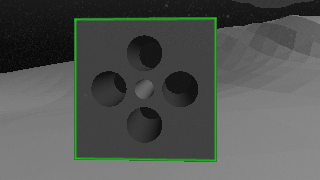
\includegraphics[width=4.5cm]{detection/clickDetLeft.png}
	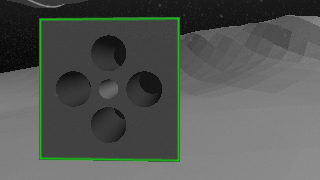
\includegraphics[width=4.5cm]{detection/clickDetRight.png}\\
	\vspace{30px}
	
	\textbf{Find Square Method}\\
	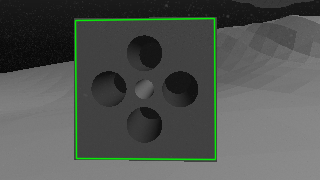
\includegraphics[width=4.5cm]{detection/squareDetLeft.png}
	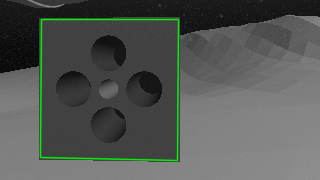
\includegraphics[width=4.5cm]{detection/squareDetRight.png}\\
	\vspace{30px}
		
	\textbf{Template Matching Method}\\
	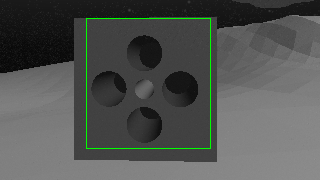
\includegraphics[width=4.5cm]{detection/tempDetLeft.png}
	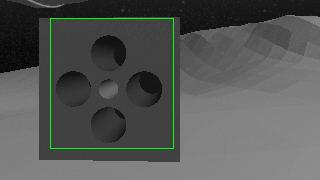
\includegraphics[width=4.5cm]{detection/tempDetRight.png}
	
	\caption[Hole Detection results with the three different methods]{Results of the three different detection method. The green rectangle is the estimate position of the square. The output of the detection step are the four corners of the green rectangle.}
	\label{fig:detectResults}
\end{figure}

As said, the Template Matching is less precise than the first method.\\
Apart this, it has different problems than previous. Firstly, if the face is viewed from a different angle, an other template image is needed, with an orientation similar to what the robot is seeing. In general, lot of template images at different angles are needed. Otherwise, some processing of the template image is necessary to orient it in a different way.\\

Secondly, the orientation can make the face to be a distorted square in the 2D image. With the first method, contours are followed well even if the quadrilateral is not a perfect square (until a certain point obviously). With the Template Matching, the only way to find the corners is by building a shape equal to the template around the similarity point. So, the real edges can be followed badly and the resultant corners can be imprecise (as can be seen in figure \ref{fig:detectResults}).\\

A better quality of the Template Matching method respect to the other is that it can be used for different shapes, not only rectangle ones. Plus, the object to be found can be also a complicated one, full of details that would put a \enquote{geometric shapes detector} (like the Find Square) in big difficulties.\\


\section{Tracking}
\label{sec:visTracking}
\textit{Object Tracking} means to follow the motion of an object of interest during time. Both the object and the camera can be mobile, even if, in this case, only the cameras move (actually, the robot moves with the cameras rigidly attached to its body). Tracking an object is usually done to estimate its pose respect to the camera frame.\\

In this work, we speak about a \textit{markerless} \textit{model-based} tracking. Thus, no markers attached to the object are needed but the object structure must be known. In this scenario, it is sufficient to give to the algorithm the 3D dimensions of the cuboid structure of the hole (i.e., the position of the eight corners respect to the object frame), and the hole's dimension and position in the front face (i.e. position of three points which describe the circumference respect to the object frame).\\
The library chosen for the tracking phase, \href{https://visp.inria.fr/}{ViSP} [\cite{visp}], uses an own format called \textit{.cao}, which syntax is described in the library  \href{https://visp-doc.inria.fr/doxygen/visp-daily/tutorial-tracking-mb-generic.html#mb_generic_advanced_cao}{documentation}.\\
As explained in section \ref{sec:visDetect}, the tracking algorithm must also know the 2D-3D correspondence of \textit{at least} four points belonging to the object. In the experiments, the provided ones are the 4 corners of the front face.\\

Three different trackers have been implemented: a \textit{Mono Cameras Tracker} (section \ref{subsec:monoTrack}), a \textit{Stereo Camera Tracker} (section \ref{subsec:stereoTrack}), and a \textit{Stereo Depth Camera Tracker} (section \ref{subsec:depthTrack}). Results and comparison of them are discussed in \mbox{section \ref{subsec:trackResult}}.\\

A tracker is linked to each camera. For RGB cameras, it can be of three types: \textit{edge-based} [\cite{visp-edge}], \textit{keypoint-based} [\cite{visp-klt}] or a mix of both. During the experiments, the hybrid method emerged as the most precise, so all the results in section \ref{subsec:trackResult} refer to this one.\\
For the depth camera used in the Stereo Depth Camera tracking, the tracker's type can be \textit{normal} or \textit{dense} [\cite{visp-depth}]. Being the \textit{dense} one more robust, it is the chosen one for the trials. Please note that it is also computationally heavier for larger matrix computations, but speed performance is not considered here.

\subsection{Two Mono Cameras Tracking}
\label{subsec:monoTrack}
This method derives from the ViSP tutorial \textit{markerless generic model-based tracking using a colour camera}  (\url{https://visp-doc.inria.fr/doxygen/visp-daily/tutorial-tracking-mb-generic.html}).\\

The implementation is straightforward: after setting the trackers (i.e. giving edge detection and keypoint detection parameters, camera parameters, and 2D-3D correspondences of the four corners), at each loop the tracker estimates the transformation matrix between each camera and the object.\\

In this method, the left and the right cameras are independent. Thus, each one provides a different pose estimation. It is not so easy to understand when one camera provides better results that the other, without taking the real pose as benchmark. So, in the applications could be difficult to choose one pose or the other. A good compromise could be to do a mean of them.\\

\subsection{Stereo Camera Tracking}
\label{subsec:stereoTrack}
This method derives from the ViSP tutorial \textit{Markerless generic model-based tracking using a stereo camera} (\url{https://visp-doc.inria.fr/doxygen/visp-daily/tutorial-tracking-mb-generic-stereo.html}).\\

The code is analogous to the previous one, except that in this case also the relative pose between each camera must be provided. If this is unknown, some method for stereo calibration must be used. Due to the fact that now the cameras are not independent, a unique pose is provided, that, as we will see later, has better precision than the previous one.

\subsection{Stereo Depth Camera Tracking}
\label{subsec:depthTrack}
This method derived from the ViSP tutorial \textit{Markerless generic model-based tracking using a RGB-D camera} (\url{https://visp-doc.inria.fr/doxygen/visp-daily/tutorial-tracking-mb-generic-rgbd.html}).\\

This method is similar to the previous one, except that now the right camera is a depth one, thus it provides range images.\\
The functions used for the depth images need the support of another library, \href{http://www.pointclouds.org/}{PCL} [\cite{pclLib}].\\
Another difference is that the depth camera does not need to initialize the 2D-3D correspondences, so the \textit{Detection} step has to be done only for the left camera.

\subsection{Tracking Results}
\label{subsec:trackResult}

In this section, performances of the three trackers are evaluated. For each one, the three different types of detection initialization (explained in section \ref{sec:visDetect}) are considered to evaluate the effects of detection's error on each kind of tracker.\\

Experiments have been conducted with a lot of simplifications: no disturbances, no camera distortions, very good visibility, nice object shape. Results described here can give only an idea on how to proceed in a more realistic environment.\\

In the scenario, the robot is perfectly still while it is tracking the object, even if the tracking methods can be used with moving objects and/or moving cameras. The vehicle is positioned in front of the square face, slightly on the right. The original images taken from cameras are cut to delete a region where a part of the vehicle is visible. This is done to make this part to not cause useless disturbances to the vision algorithms. In the depth images, this is not necessary, because there is no interference.\\

In figure \ref{fig:photoTracking} the detected shape and the estimated frame are drawn on the camera images. Differences are barely visible when comparing the first two initialization methods (the ideal one and the Find Square one) in all the three tracking methods.\\

Instead with the Template Matching detection initialization (last group of images of figure \ref{fig:photoTracking}), the lower precision (visible in figure \ref{fig:detectResults}) is paid in tracking results, especially in the depth case. This is clearer in figure \ref{fig:templateErrors} where the error is plotted. With this initialization, the depth-stereo method is even worse than the monocular case.\\
This can be due to the fact that the depth image is not initialized with 2D-3D correspondence; thus we pay more the initialization error, being done only in the left image.\\
This demonstrates that it is not always better to have a stereo RGB-D camera instead of a normal stereo RGB. This is an interesting result and should be further explored with more realistic scenes.\\

\begin{figure}[H]
	\begin{center}
		\textbf{Already known coordinates Initialization}
	\end{center}
	\vspace{-10px}	
   	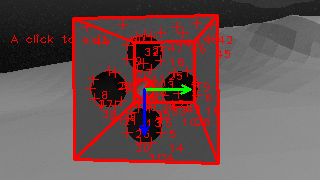
\includegraphics[width=3.4cm]{tracking/click/mono_left.png}
	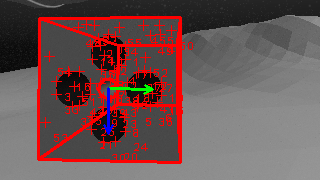
\includegraphics[width=3.4cm]{tracking/click/mono_right.png}
	\hspace{10px}
	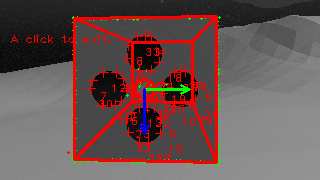
\includegraphics[width=3.4cm]{tracking/click/stereo_left.png}
	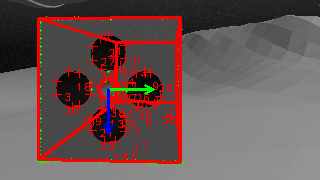
\includegraphics[width=3.4cm]{tracking/click/stereo_right.png}\\
	{\footnotesize \hspace*{20px}\textit{Mono Cameras Case} \hspace{120px} \textit{Stereo Cameras Case}}\\
	\centering{
		
	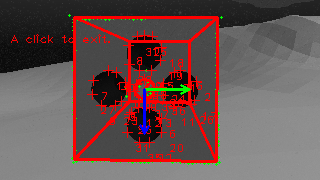
\includegraphics[width=3.4cm]{tracking/click/depth_left.png}
	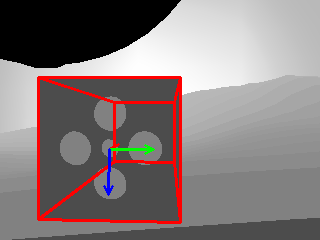
\includegraphics[width=3.4cm]{tracking/click/depth_right.png}}\\
    {\footnotesize \textit{Stereo Depth Camera Case}}\\  
\end{figure}
\vspace{-12px}
\begin{figure}[H]
	\begin{center}
		 \textbf{Find Square Initialization}
	\end{center}
	\vspace{-10px}
	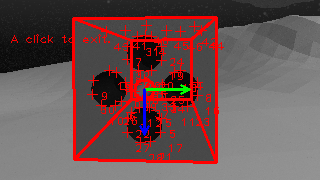
\includegraphics[width=3.4cm]{tracking/square/mono_left.png}
	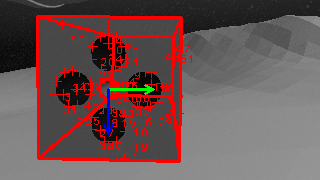
\includegraphics[width=3.4cm]{tracking/square/mono_right.png}
	\hspace{10px}
	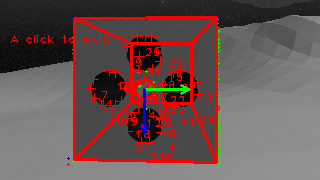
\includegraphics[width=3.4cm]{tracking/square/stereo_left.png}
	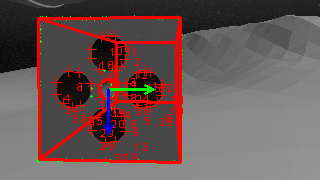
\includegraphics[width=3.4cm]{tracking/square/stereo_right.png}\\
	{\footnotesize \hspace*{20px}\textit{Mono Cameras Case} \hspace{120px} \textit{Stereo Cameras Case}}\\
	\centering{
		
	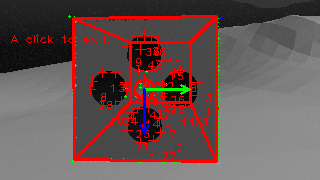
\includegraphics[width=3.4cm]{tracking/square/depth_left.png}
	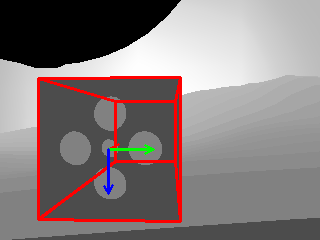
\includegraphics[width=3.4cm]{tracking/square/depth_right.png}}\\
    {\footnotesize \textit{Stereo Depth Camera Case}}\\  
\end{figure}
\vspace{-12px}
\begin{figure}[H]
	\begin{center}
		\textbf{Template Matching Initialization}
	\end{center}
	\vspace{-10px}
	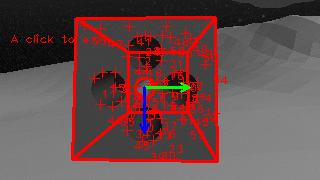
\includegraphics[width=3.4cm]{tracking/templ/mono_left.png}
	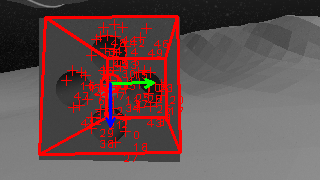
\includegraphics[width=3.4cm]{tracking/templ/mono_right.png}
	\hspace{10px}
	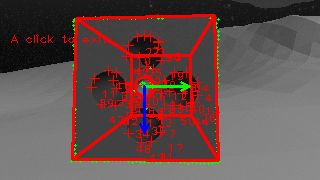
\includegraphics[width=3.4cm]{tracking/templ/stereo_left.png}
	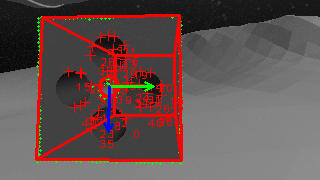
\includegraphics[width=3.4cm]{tracking/templ/stereo_right.png}\\
	{\footnotesize \hspace*{20px}\textit{Mono Cameras Case} \hspace{120px} \textit{Stereo Cameras Case}}\\
	\centering{
		
	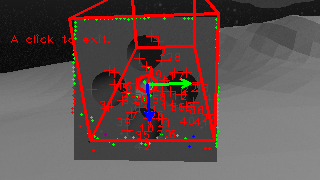
\includegraphics[width=3.4cm]{tracking/templ/depth_left.png}
	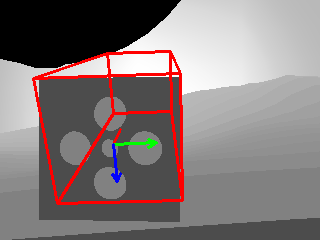
\includegraphics[width=3.4cm]{tracking/templ/depth_right.png}}\\
    {\footnotesize \textit{Stereo Depth Camera Case}}\\
\end{figure}
\begingroup
\captionof{figure}[Tracking results with the three different detection initializations]{Results of the three tracking methods with the three detection initializations. Red lines are the contours of the model which represents where the object is estimated to be; little red $+$ marks are the points detected by the keypoint algorithm. Green dots are the tracked correspondent points between the left and the right images, in fact they are present only in the stereo cases. The arrows represent the estimated object frame: green for y-axis, blue for z-axis, red for x-axis (which goes inside the hole and it is barely visible).}
\label{fig:photoTracking}
\endgroup
\vspace{60px}

With the two good initializations (the ideal one and the Find Square one), the two stereo methods have similar results, overall better than the mono case. This is visible in the errors' plots of figure \ref{fig:clickErrors} and figure \ref{fig:squareErrors}. Anyway, we can also see that the mono camera case has not so bad performance. Considering that a stereo camera is much more expensive, a tracking with a single mono camera can be an advisable deal.\\

Another interesting outcome for the monocular case, is that the position of the camera influences the results. This is because different view angles provide different tracking performance.\\

In the plots of the errors (fig. \ref{fig:clickErrors}, fig. \ref{fig:squareErrors}, and fig. \ref{fig:templateErrors}), a lot of variations can be seen while the time goes on, although the robot and the object are still. This is due to the nature of the tracking algorithm, which continuously updates the pose at each new image received by the camera. Anyway, it must be noticed that the variations are little for both the linear and the angular parts. So, taking the pose at a certain time instead of an another is not so influential.\\

\begin{figure}
	\centering
	\textbf{Already known coordinates Initialization}\\
	\vspace*{20px}
	\centerline{
		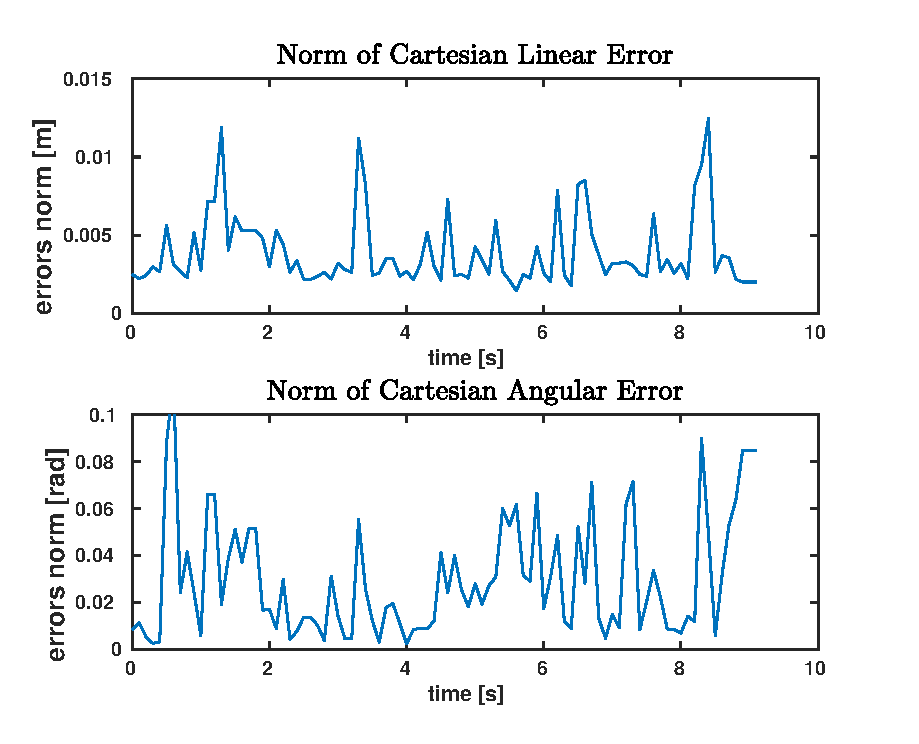
\includegraphics[width=9cm]{tracking/click-mono-left.eps}
		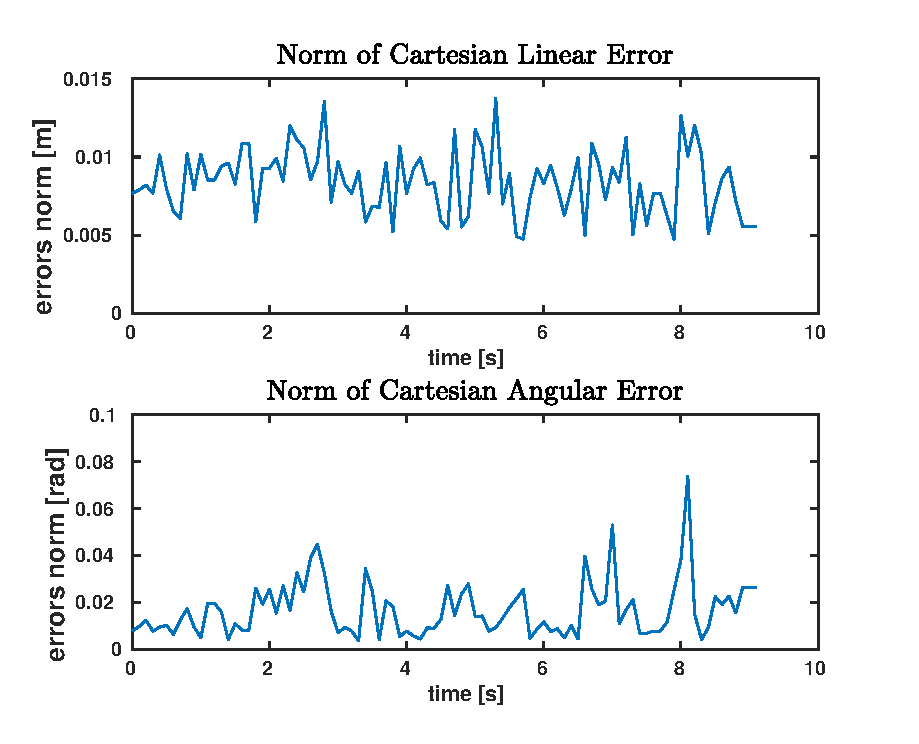
\includegraphics[width=9cm]{tracking/click-mono-right.eps}
	}
	\hspace*{15px}\textit{Mono (left Camera) Case} \hspace{125px} \textit{Mono (right Camera) Case}\\
	\vspace{30px}
	\centerline{
		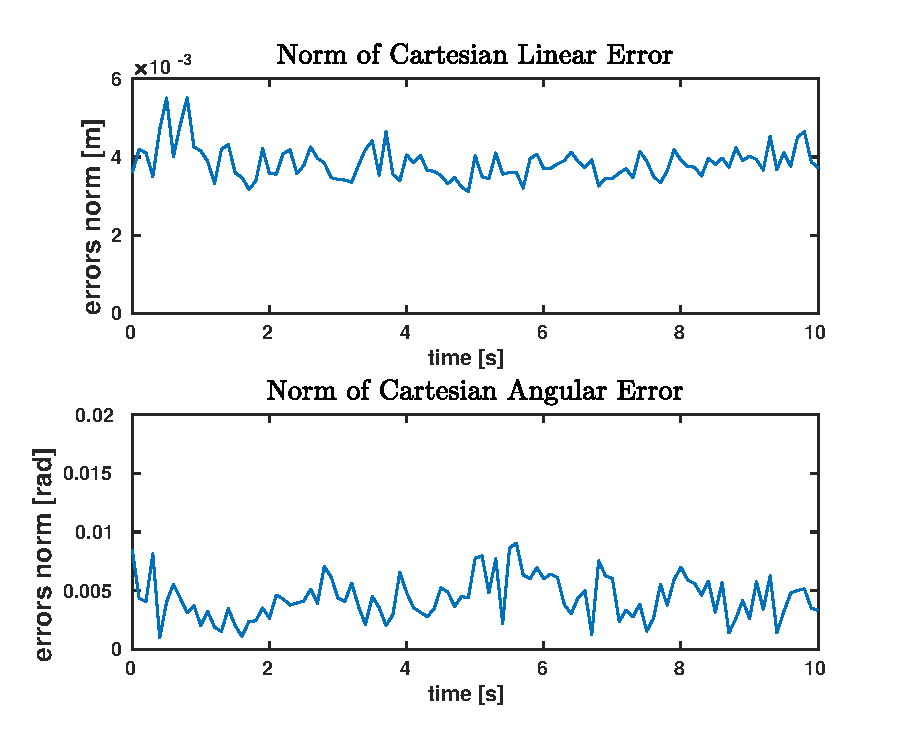
\includegraphics[width=9cm]{tracking/click-stereo.eps}
		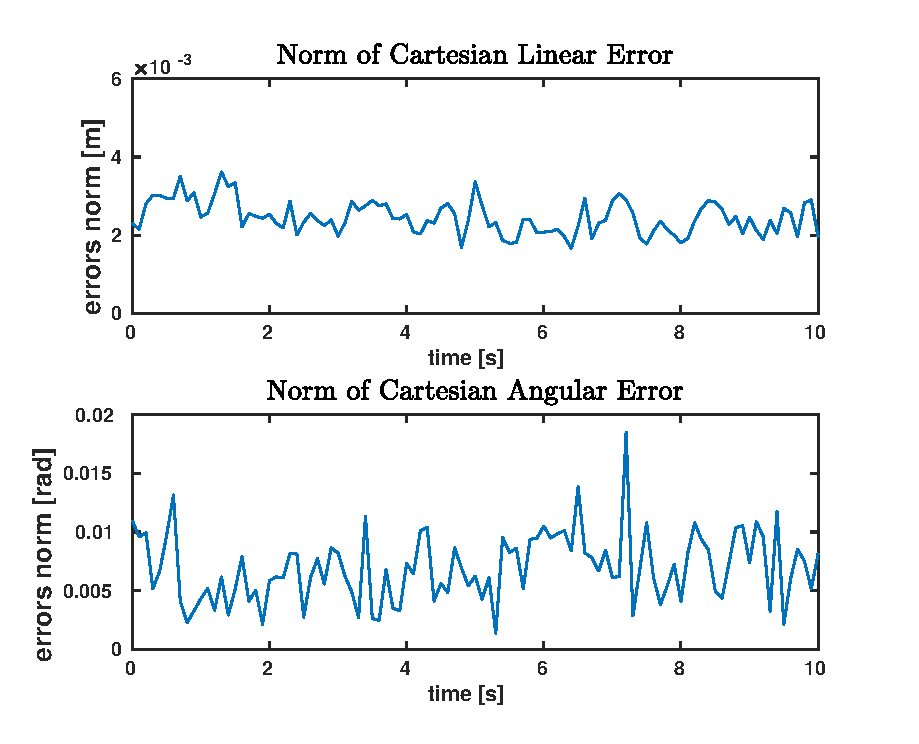
\includegraphics[width=9cm]{tracking/click-depth.eps}
	}
	\hspace*{20px}\textit{Stereo Camera Case} \hspace{135px} \textit{Stereo Depth Camera Case}\\
	\vspace{30px}
	\caption[Tracking error plots with ideal detection initialization]{Linear and angular error (in norm) between the true pose and the estimated one. The tracking is initialized with the ideal detection method of section \ref{subsec:clickMethod}.}
	\label{fig:clickErrors}
\end{figure}

\begin{figure}
	\centering
	\textbf{Find Square Initialization}\\
	\vspace*{20px}
	\centerline{
		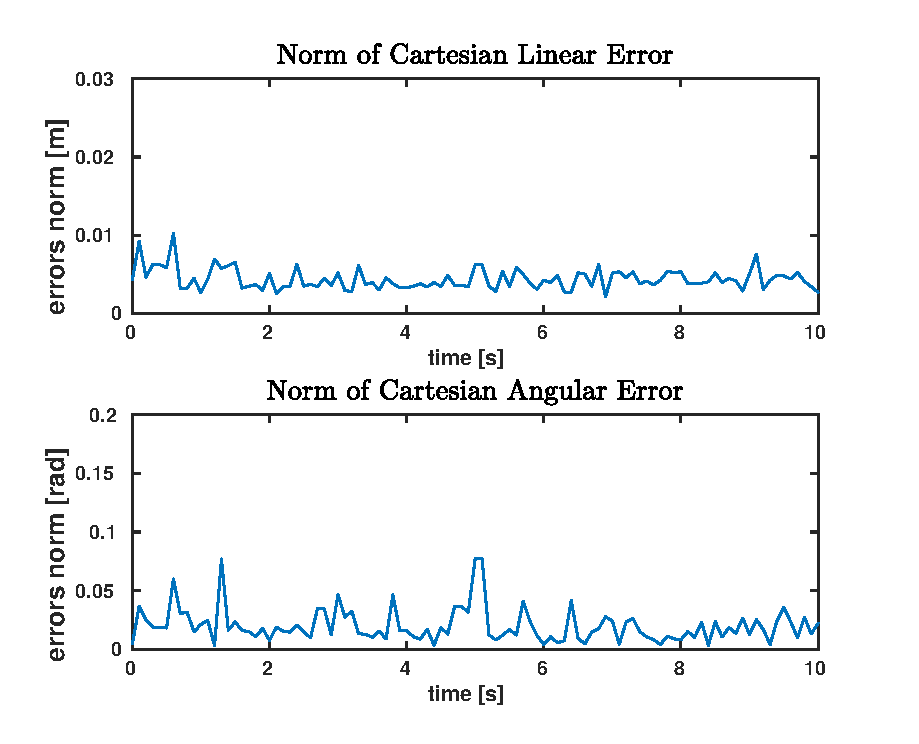
\includegraphics[width=9cm]{tracking/square-mono-left.eps}
		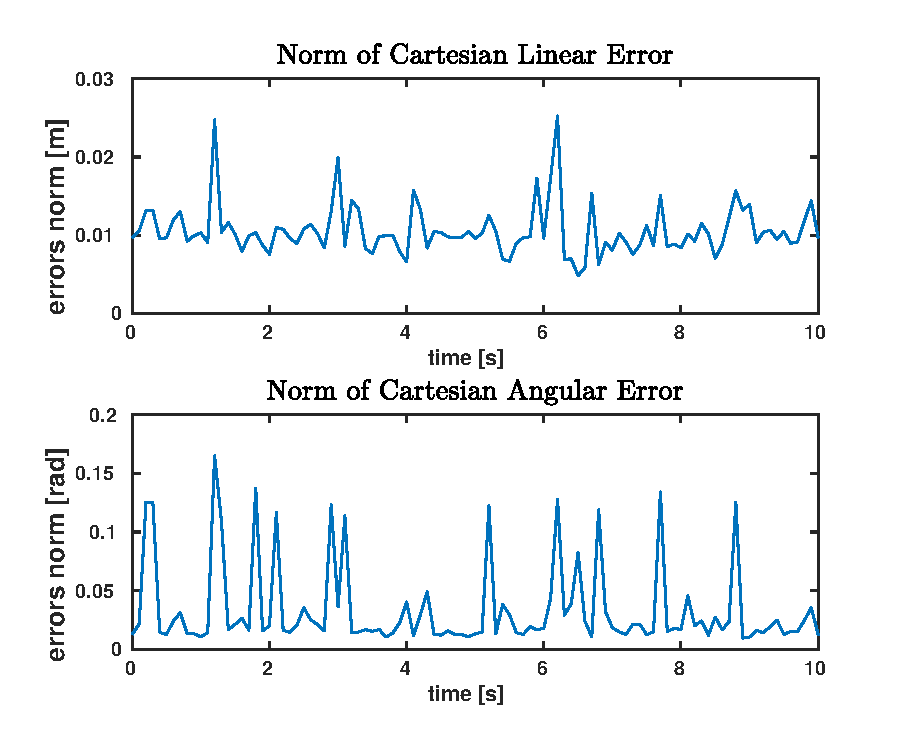
\includegraphics[width=9cm]{tracking/square-mono-right.eps}
	}
	\hspace*{15px}\textit{Mono (left Camera) Case} \hspace{125px} \textit{Mono (right Camera) Case}\\
	\vspace{30px}
	\centerline{
		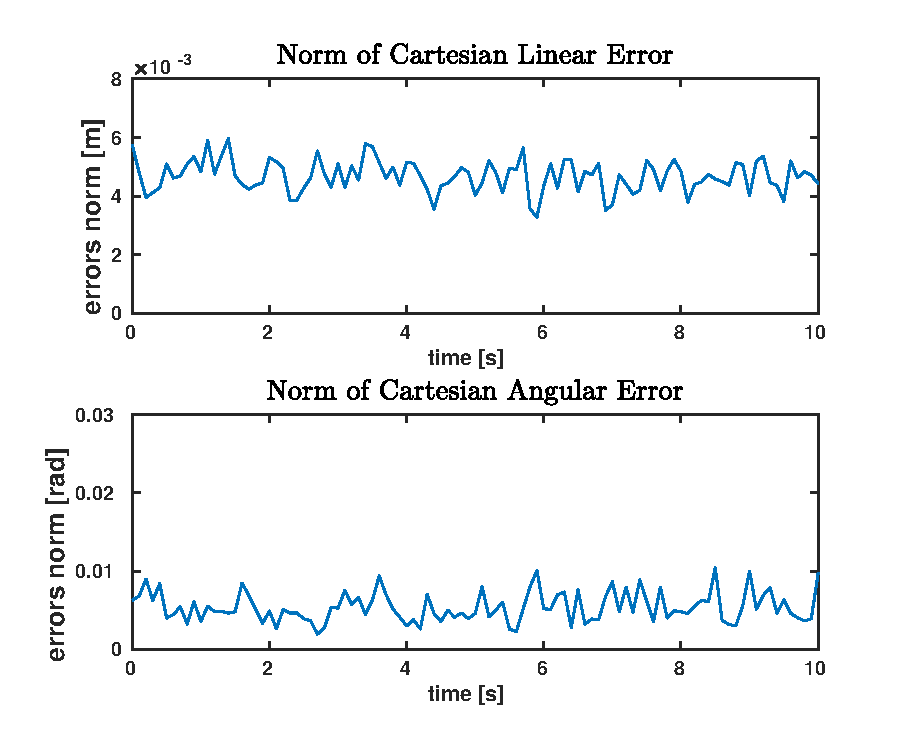
\includegraphics[width=9cm]{tracking/square-stereo.eps}
		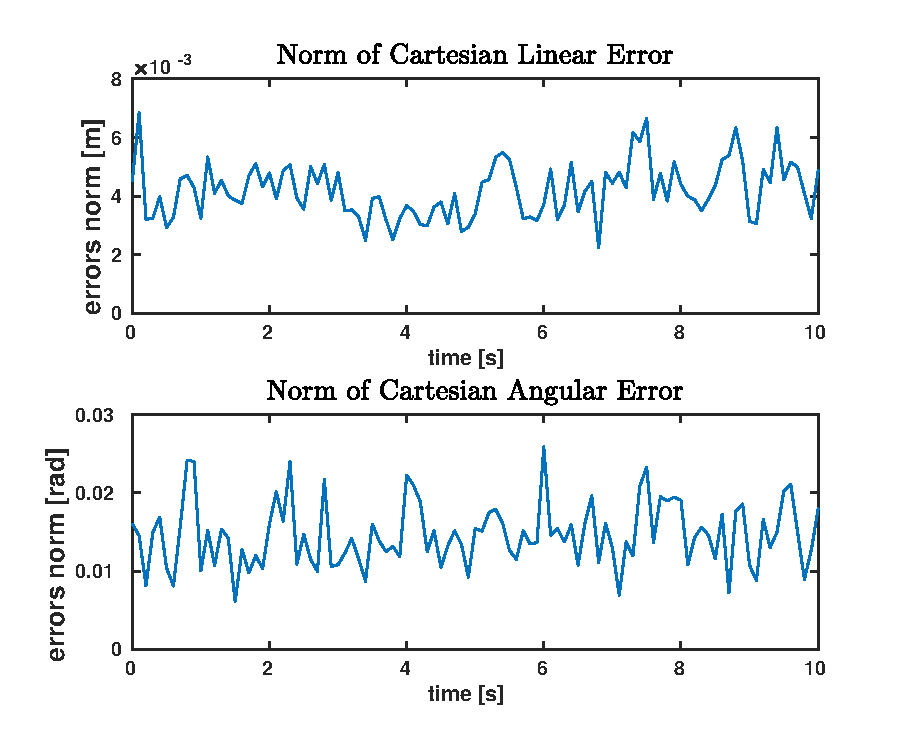
\includegraphics[width=9cm]{tracking/square-depth.eps}
	}
	\hspace*{20px}\textit{Stereo Camera Case} \hspace{135px} \textit{Stereo Depth Camera Case}\\
	\vspace{30px}
	\caption[Tracking error plots with find square detection initialization]{Linear and angular error (in norm) between the true pose and the estimated one. The tracking is initialized with the Find Square detection method of section \ref{subsec:findSquare}.}
	\label{fig:squareErrors}
\end{figure}

\begin{figure}
	\centering
	\textbf{Template Matching Initialization}\\
	\vspace*{20px}
	\centerline{
		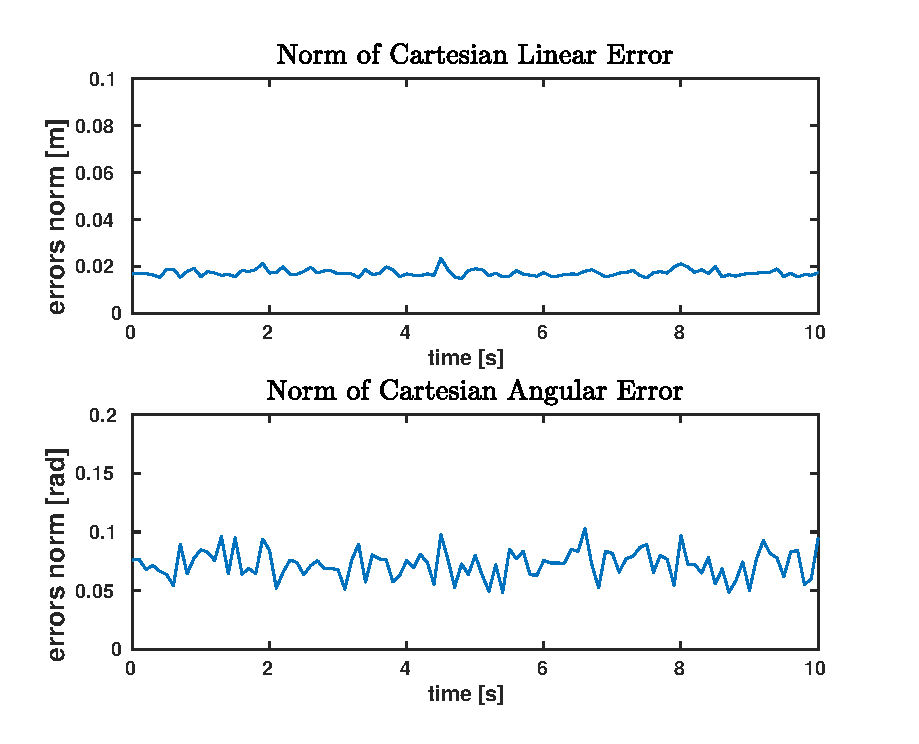
\includegraphics[width=9cm]{tracking/templ-mono-left.eps}
		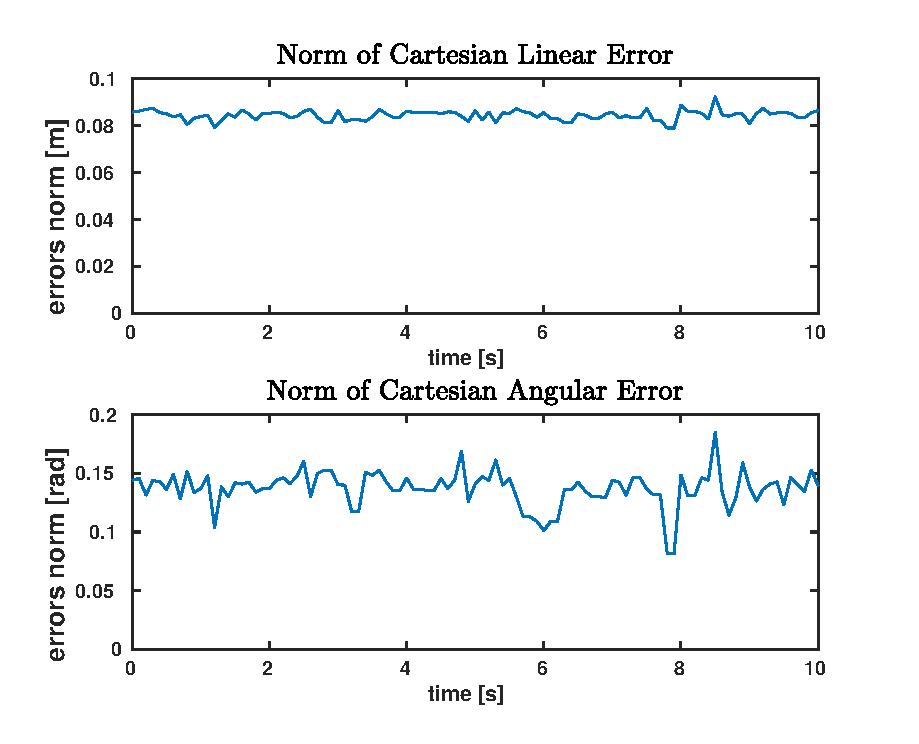
\includegraphics[width=9cm]{tracking/templ-mono-right.eps}
	}
	\hspace*{15px}\textit{Mono (left Camera) Case} \hspace{125px} \textit{Mono (right Camera) Case}\\
	\vspace{30px}
	\centerline{
		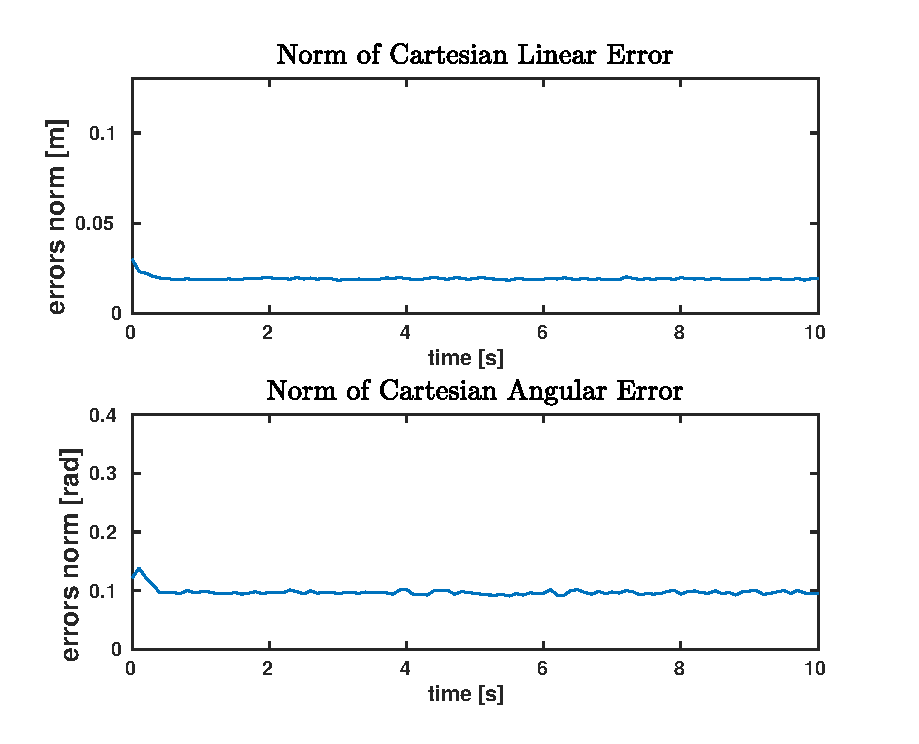
\includegraphics[width=9cm]{tracking/templ-stereo.eps}
		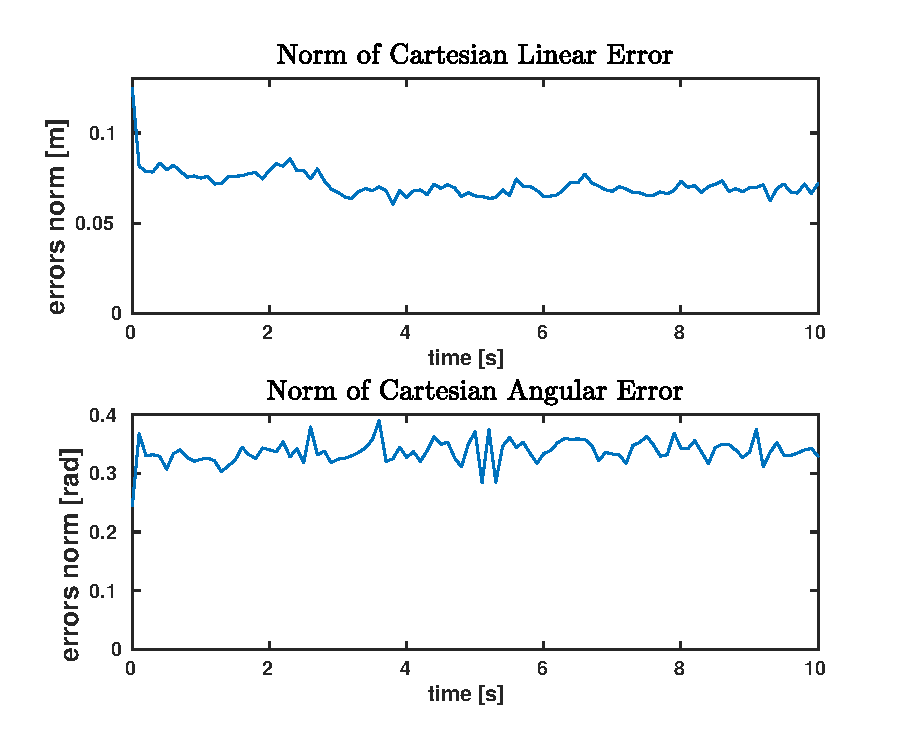
\includegraphics[width=9cm]{tracking/templ-depth.eps}
	}
	\hspace*{20px}\textit{Stereo Camera Case} \hspace{135px} \textit{Stereo Depth Camera Case}\\
	\vspace{30px}
	\caption[Tracking error plots with template matching detection initialization]{Linear and angular error (in norm) between the true pose and the estimated one. The tracking is initialized with the Template Matching detection method of \mbox{section \ref{subsec:templateMatch}}.}
	\label{fig:templateErrors}
\end{figure}